
%(BEGIN_QUESTION)
% Copyright 2013, Tony R. Kuphaldt, released under the Creative Commons Attribution License (v 1.0)
% This means you may do almost anything with this work of mine, so long as you give me proper credit

Torricelli's Theorem describes the velocity of a liquid exiting the bottom of a vessel as a function of liquid height within the vessel, and also the acceleration of Earth's gravity ($g$):

$$\includegraphics[width=15.5cm]{i02747x01.eps}$$

We also know that the hydrostatic pressure generated by a vertical column of liquid follows this formula:

$$P = \rho g h$$

Combine this formula with Torricelli's Theorem to express fluid velocity through an orifice as a function of {\it pressure} rather than of liquid {\it height}.

\underbar{file i02747}
%(END_QUESTION)





%(BEGIN_ANSWER)

In order to combine these two formulae together, we need to identify the common variable.  In this case, it is {\it height}.  Note that $g$ is not really a variable, but rather a {\it constant} so long as the location is on the surface of planet Earth.

Now that we know what the common variable is, we may manipulate the hydrostatic pressure formula to solve for that variable, so that we will have something to substitute into Torricelli's Theorem and finally have an formula solving for velocity ($v$) in terms of pressure ($P$):

$$P = \rho g h$$

$$h = {P \over \rho g}$$

\vskip 10pt

$$v = \sqrt{2 g h}$$

$$v = \sqrt{2 g \left(P \over \rho g \right)}$$

$$v = \sqrt{2 \left(P \over \rho \right)}$$

$$v = \sqrt{2 P \over \rho}$$

\centerline{(Alternatively . . .)}
 
$$v = \sqrt{2} \sqrt{P \over \rho}$$

Note that $P$ actually refers to the amount of {\it differential} pressure across the opening, since Torricelli's Theorem assumes a discharge into atmospheric pressure as well as a vented tank (atmospheric pressure on top of the liquid).

%(END_ANSWER)





%(BEGIN_NOTES)


%INDEX% Physics, dynamic fluids: Torricelli's theorem

%(END_NOTES)


